\documentclass[aspectratio=169]{beamer}
\setbeamertemplate{navigation symbols}{}
\usepackage{tikz}
\usetikzlibrary{positioning}
\usepackage{hyperref}
\usepackage{tcolorbox}
\usepackage[backend=biber]{biblatex}
\addbibresource{Documentation/Presentation/references.bib}

\usetheme{Boadilla}
\useoutertheme{tree}
\title{Kaavish \textsc{I} Presentation}
\author{Team \textsc{Prions}}
% \AtBeginSection[]
% {
%     \begin{frame}<beamer>{Outline}
%     \tableofcontents[currentsection, currentsubsection]
%     \end{frame}
% }

% \AtBeginSubsection[]
% {
%     \begin{frame}<beamer>{Outline}
%     \tableofcontents[currentsection, currentsubsection]
%     \end{frame}
% }

\begin{document}
% Title slide frame

\begin{frame}[plain]
%%%%%%%% Title slide details %%%%%%%%%%%%%%


% Background Image
\newcommand{\myBackround}
{
    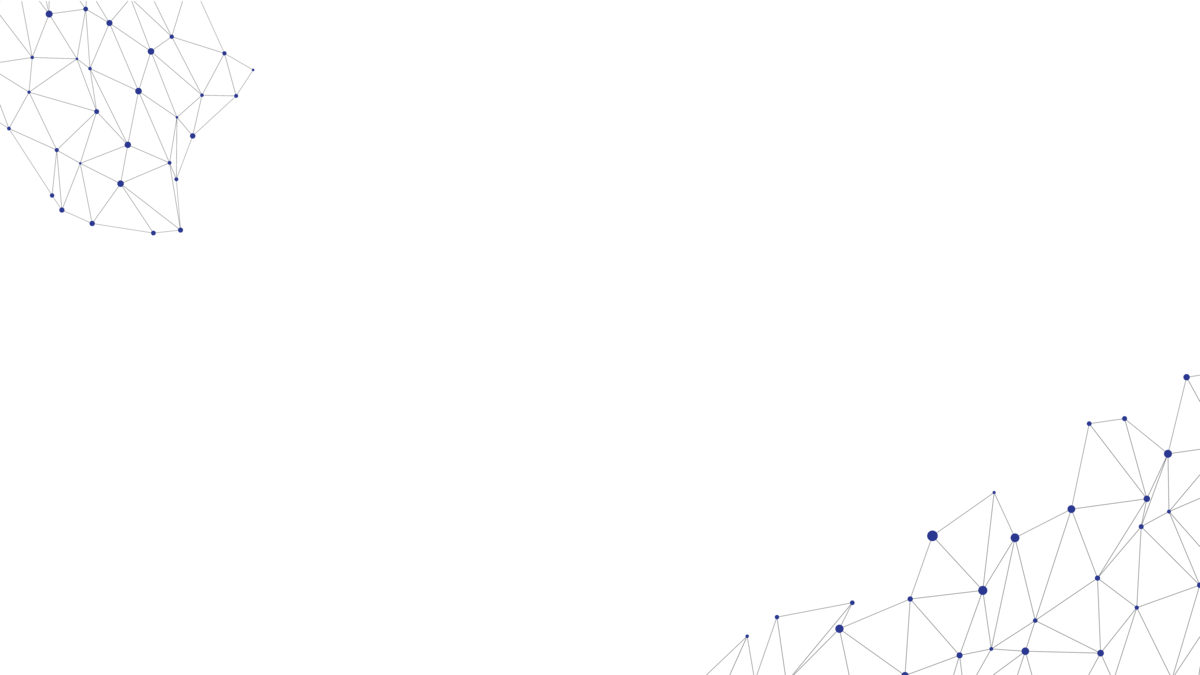
\includegraphics[width=\paperwidth]{bg.png}
}

% Title
\newcommand{\myTitle}
{
    Kavish 1 Presentation 
}

% Subtitle
\newcommand{\mySubTitle}
{
    Ali Hamza, Haris Ladhani, \\ M. Usaid Rehman \& Maham S. Patel
}

% Author
\newcommand{\myAuthor}   
{
    Team Prions
}
\newcommand{\myAffiliate}
{
  Habib University
}
% Presentation Date
\newcommand{\myDate}   
{
    \today
}
% Logo
\newcommand{\myLogo}   
{
    \includegraphics[width=1cm]{Logo.png}
}
%%%%%%%%%%%%%%%%%%%%%%%%%%%%%%%%%%%%

%%%%%%%%%% Title slide code %%%%%%%%%%%
\begin{tikzpicture}[remember picture,overlay]
% Background color

\fill[white] (current page.south west) rectangle (current page.north east);
% Background image
\node[above right,inner sep=0pt] at (current page.south west)
    {
        \myBackround
    };
    
% Title & Subtitle
\node
[
    above=0.5cm,
    align=center,
    draw=black!50,
    % rounded corners,
    double,
    double distance=0.1cm,
    double=blue!10,
    fill=yellow!10,
    inner xsep=15pt,
    inner ysep=10pt, 
    minimum width=0.7\textwidth,
    text width=0.6\textwidth
] (title) at (current page.center)
{
    \LARGE \myTitle  \\[5pt]
    \small \mySubTitle
};

% Author 
\node[ below=0.5cm] (author) at (title.south){\myAuthor};

% Author 
\node[ below=0.25cm ](affiliate) at (author.south){\small \myAffiliate};

% Date
\node[below=0.25] (date) at (affiliate.south){\large \myDate};

% Logo
\node
[
    below =0.25cm
] at (date.south)
{
    %\myLogo
};

\end{tikzpicture}
\end{frame}

\begin{frame}{Outline}
\tableofcontents
\end{frame}

\section{Introduction}

\subsection{Protein Interactions \& Protein Complexes}
\begin{frame}{Protein Interactions \& Protein Complexes}
    \begin{itemize}
        \item Proteins are essential nutrients of body that carry out cellular activities
        \item Protein-Protein Interaction occurs when two or more proteins come into a physical contact
        \item Protein Complexes are multimolecular machines that bind by protein protein interactions
        \item Protein Complexes play a huge role in biological systems and perform functions such as DNA transcription and mRNA translation
    \end{itemize}
\end{frame}

\subsection{Problem Statement}
\begin{frame}{Problem Statement}
\begin{tcolorbox}
    PPI Network data is \textit{noisy and incomplete}, often contains \textit{false-positives}, and present algorithms are limited in their scope and overlook certain properties, e.g. unable to account \textit{small and sparse} protein complexes. PPI Networks are also represented as static objects which leads to oversimplification of complex biological features.
\end{tcolorbox}
\end{frame}

\subsection{Proposed Solution}
\begin{frame}{Proposed Solution}
\begin{tcolorbox}
    Our proposed solutions involves incorporating data from multiple sources and then making use of an \textit{ensemble clustering framework} to account for algorithmic limitations and incorporate further biological information into our PPI networks through the use of \textit{dynamic} PPI networks.
\end{tcolorbox}
\end{frame}

\section{Literature Review}
\subsection{Protein-Protein Interaction Networks}
\begin{frame}{Protein-Protein Interaction Networks}
\begin{itemize}
    \item A large number of proteins interacting forms a network of interactions 
    \item This network can be modelled
    \item These networks have proteins as nodes and interactions as edges 
    \item These PPI networks are akin to social networks
    \item Standard network analysis and graph theoretical methods can be applied 
    to gain insight
\end{itemize}
\end{frame}

\begin{frame}{Static \& Dynamic PPI Network}
\begin{itemize}
    \item Static Networks 
    \begin{itemize}
        \item Simple graph representations
        \item Screenshots of PPI Network at a point in time
        \item Results in loss of important biological information
    \end{itemize}
    \item Dynamic Networks
    \begin{itemize}
        \item Dynamic graphs that change over time
        \item Carry out real world biological protein functions
        \item Makes use of probabilistic models
    \end{itemize}
\end{itemize}
    
\end{frame}

\begin{frame}{Features of PPI Networks}

\begin{itemize}
    \item Topological Features
    \begin{itemize}
        \item Degree Centrality
        \item Closeness Centrality
        \item Betweeness Centrality
        \item Clustering Coefficient
        \item Average Degree
        \item Density
    \end{itemize}
    \item Biological Features
    \begin{itemize}
        \item Interaction Scores
    \end{itemize}
\end{itemize}
    
\end{frame}

\subsection{Protein Complex Prediction Methods}
\begin{frame}{Protein Complex Prediction Methods}
    \begin{itemize}
        \item These clusters are subgraphs with their own topological properties
        \item There are several methods to find clusters in PPIs
        \item If these methods are used in isolation, the clusters are themselves complexes
        \item These methods can be broadly classified into two categories:
            \begin{itemize}
                \item Cluster-quality-based methods
                \item Node-affinity-based methods
            \end{itemize}
    \end{itemize}
\end{frame}

\begin{frame}{Protein Complex Prediction Methods}{Cluster-quality-based methods}
    \begin{itemize}
        \item Define cluster quality functions and design corresponding algorithms to extract clusters
        \item Cluster quality functions can be divided into local-cluster-quality functions and global-cluster-quality functions 
        \item Local-cluster-quality functions measure individual clusters. Corresponding methods identify individual clusters with optimal local-cluster-quality.
        \item Global-cluster-quality functions measure all clusters by considering them as a whole. 
        \item Corresponding methods search for an optimal set of clusters with the best global-cluster-quality value
    \end{itemize}
\end{frame}

\begin{frame}{Protein Complex Prediction Methods}{Node-affinity-based methods}
    \begin{itemize}
        \item Cluster-quality methods ignore the relationship among nodes 
        \item Node-affinity-based methods generate clusters by expanding neighbors with high-affinity scores
        \item Local-node-affinity functions measure the local neighborhood affinity between nodes
        \item Global-node-affinity functions measure the global network affinity between nodes
        \item Local-node-affinity measures can vary and make use of different properties of nodes and edges
    \end{itemize}
\end{frame}

\begin{frame}{Protein Complex Prediction Methods}{Examples}
\begin{center}
    \begin{tabular}{c|c}
        Algorithm & Category \\
        \hline \\
        NCMine & Local-cluster-quality-based method \\
        Core\&Peele & Local-cluster-quality-based method \\
        CFinder & Local-node-affinity-based method \\ 
        SPICi & Local-node-affinity-based method \\
        RSGNM & Global-cluster-quality based method \\
        MCL & Global-node-affinity based method
    \end{tabular}
\end{center}
\end{frame}

\begin{frame}{Challenges in Protein Complex Prediction}
    \begin{itemize}
        \item Finding protein complexes is an NP-complete problem, which means that 
        approximate or heuristic solutions have to be found 
        \item There are many factors to consider while designing a method because of the numerous topological and biological properties 
        \item Finding the right features upon which to base the clustering algorithm is a challenge
        \item Most clustering methods only work for certain protein complexes, and not for others
    \end{itemize}
\end{frame}

\begin{frame}{Ensemble Clustering Methods}
\begin{itemize}
    \item In \textbf{Consensus Clustering}, base clusters are fused with different approaches to generate a consensus matrix which yields a final set of complexes.
    \item Another method is, \textbf{Meta-Clustering}. Here we do a further interpretation of the base clusters by considering each base cluster as a unit.
    \item These units are considered as nodes in a completely weighted graph. The edges are the normalized Pearson correlation between the nodes. 
\end{itemize}
\end{frame}


\subsection{Data \& Databases}
\begin{frame}{Data \& Databases}
Extracted datasets for humans from the following primary and secondary databases:
    \begin{table}[htpb]
      \centering
      \vspace{1 em}
      \label{tab:dataset1}
      \begin{tabular}{l|l}
      \hline
      Name & Website \\
      \hline
      DIP & \url{http://dip.doe-mbi.ucla.edu/dip/Main.cgi}\\
      BioGRID & \url{https://thebiogrid.org/} \\
      APID & \url{http://cicblade.dep.usal.es:8080/APID/init.action}\\
      HPRD & \url{http://www.hprd.org/} \\ 
      MINT & \url{https://mint.bio.uniroma2.it}\\
      STRING & \url{https://string-db.org/} \\
    \hline
    \end{tabular}
  \end{table}
\end{frame}

\begin{frame}{Method of Compilation}
    \begin{enumerate}
        \item Extract list of human proteins from uniprot; an online database for protein sequencing
        \item Query and extract list of human protein-protein interactions from the repositories mentioned earlier
        \item Convert the extracted files from the previous step into tsv's
        \item Iterate through files and add the necessary components of interactions to our database
        \item Filter database to remove unnecessary or incomplete data
        \item Add MINT scores for those interactions that are extracted from repositories not obtained from MENTHA or MINT
    \end{enumerate}
\end{frame}

\begin{frame}{Method of Compilation}{Diagram}
\begin{figure}[h!]
    \centering
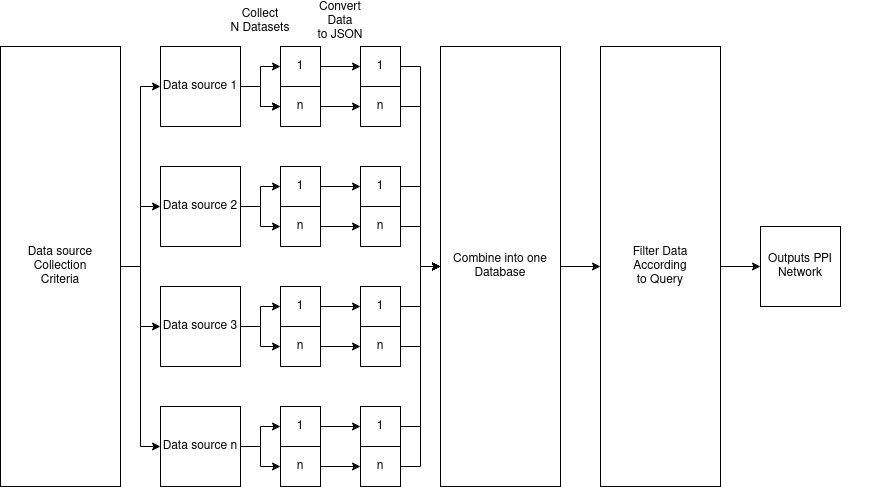
\includegraphics[scale=0.3]{Documentation/Presentation/data-pipeline.png}
\caption{Database Compilation Pipeline.}
\label{fig: data_pipelinediag}
\end{figure}
\end{frame}

\begin{frame}{Structure of Datasets}
Extracted human PPIN datasets from repositories cleaned to provide the following for each interaction:
    \begin{itemize}
        \item \textbf{UniprotKB IDs}: Unique universal identifier for the proteins as stored in the UniProt database.
        \item \textbf{Gene Names}: Recommended name used for representing the genes, adhering to the gene nomenclature.
        \item \textbf{MINT score}: Score between 0 and 1 assigned to the interaction pair according to the cumulative experimental evidence and publications supporting the existence of the interaction.
        
    \end{itemize}
\end{frame}


\section{SDS, SRS, \& Prototype}
\subsection{Database}
\begin{frame}{Database}
    We created a non-relational database using MongoDB with the following collections inside the database:
    \begin{table}[htpb]
      \centering
      \vspace{1 em}
      \label{tab:database}
      \begin{tabular}{l|l}
      \hline
      Collection & Description \\
      \hline
      Proteins & Proteins sourced from databases\\ 
      Interactions & Sourced from various sources\\
      Taxonomy & Species of interactions\\ 
      Experimental Details & Experimental details of interactions \\
    \hline
    \end{tabular}
  \end{table}
\end{frame}

\begin{frame}{ERD}
    \begin{figure}[h!]
    \centering
    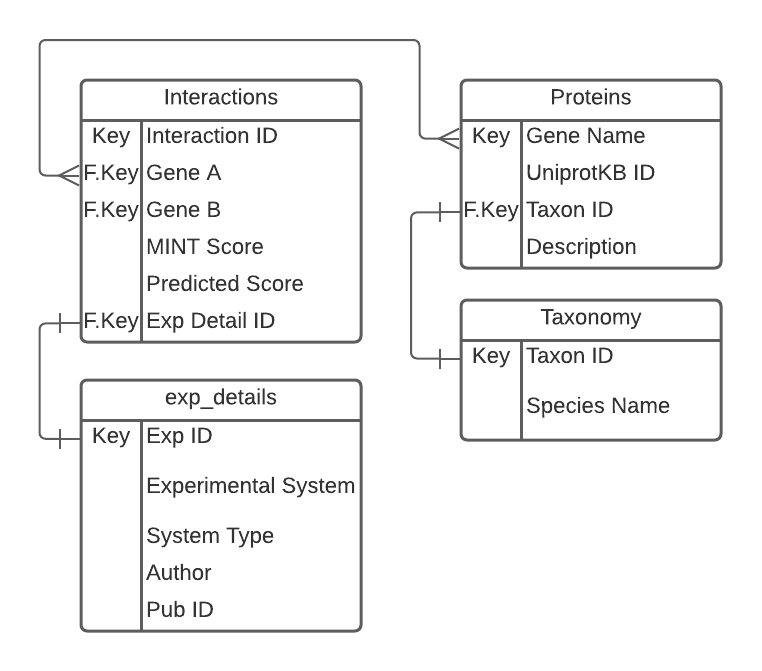
\includegraphics[scale=0.6]{Documentation/Presentation/ERD.png}
    \caption{ERD Diagram.}
    \label{fig: ERD}
    \end{figure}
\end{frame}

\subsection{Proposed System Model}
\begin{frame}{Proposed System Model}
\begin{figure}[h!]
    \centering
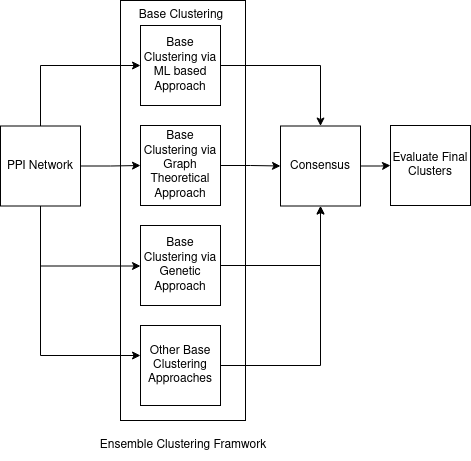
\includegraphics[scale=0.4]{Documentation/Presentation/algo-pipeline.png}
\caption{Proposed PPI Prediction Pipeline.}
\label{fig: algo_pipelinediag}
\end{figure}
\end{frame}



\begin{frame}{Evaluation Metrics}
    Some common evaluation metrics are:
    \begin{itemize}
        \item Precision -- fraction of relevant instances among the retrieved instances
        \item Recall -- fraction of relevant instances that are successfully retrieved 
        \item F-measure -- harmonic mean of precision and recall 
        \item Sensitivity -- measure of proteins that are common in given (known) complexes and identified clusters 
        \item Positive Predictive Value (PPV) -- the proportion of true positives in terms of proteins themselves
        \item Accuracy (Acc) -- square root of PPV and sensitivity
    \end{itemize}
\end{frame}

\section{Limitations, and Adaptive Measures}
\begin{frame}{Limitations, and Adaptive Measures}
    \begin{enumerate}
        \item Lack of uniformity in current data sources.
        \item Size of present data despite being incomplete and erroneous.
        \item Lack of expert advice.
        \item Novelty of idea.
    \end{enumerate}
\end{frame}

\section*{Idea Publication}
\begin{frame}{Idea Publication}
    \begin{columns}
    % Column 1
        \begin{column}{0.5\textwidth}
                Poster publication for the project idea at the Aga Khan University (AKU) Biological Science Research Symposium held by Department of Biological and Biomedical Sciences on 15th December, 2021.
        \end{column}
        % Column 2    
        \begin{column}{0.5\textwidth}
            \begin{figure}
            \centering
                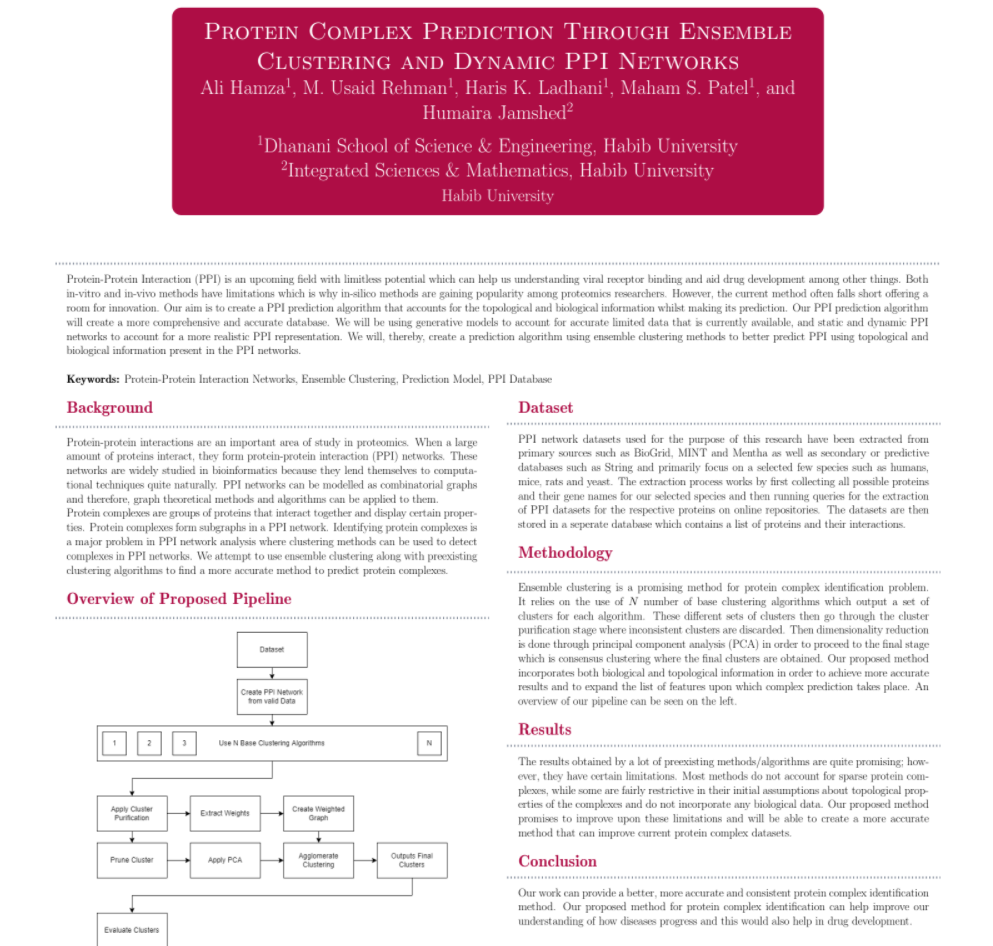
\includegraphics[width=0.75\textwidth]{Documentation/Presentation/publication.PNG}
                \caption{Poster Publication}
            \end{figure}
        \end{column}
    \end{columns}
\end{frame}

\section{References}

\begin{frame}[allowframebreaks]{References}
    \nocite{*}
    \printbibliography
\end{frame}
    


\end{document}